
In this section, we present experiments in which the Plane-Tree 3D model and 3D reconstruction data compression system are examined. The Plane-Tree is first compared to its similar neighbour method, the Octree. It is compared with the Octree using the mean error metric discussed in section \ref{metricsSection}. The two algorithms are compared when compressing three commonly available object models, Bunny, Fandisk and Horse. These data are shown in Figure \ref{fig:MODELSUSEDA}. \\

\begin{figure}[!htb]
\centering
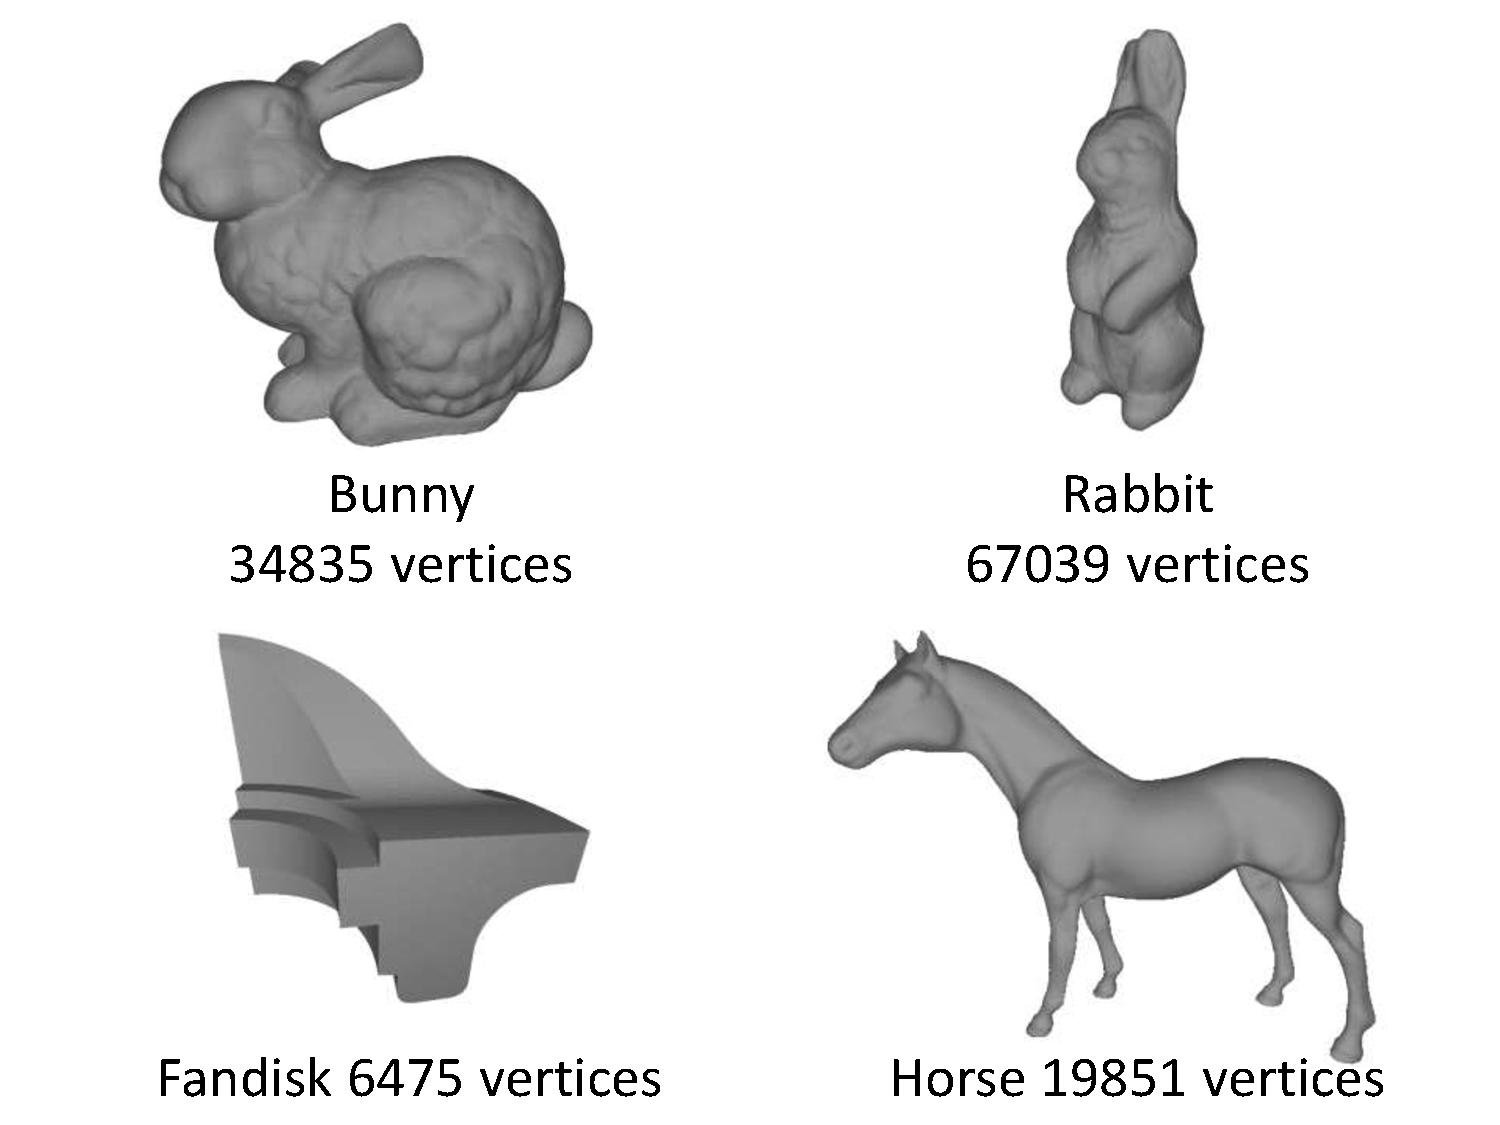
\includegraphics[width=4.0in]{images/experiments/test_data/modelsused}
\caption{Models used to assess the Plane-Tree compression algorithm.}
\label{fig:MODELSUSEDA}
\end{figure}


Next, the Plane-Tree is compared with the current state-of-the-art methods from 3D object compression research. These experiments are presented in section \ref{SEC:PTVSSOTA}. These experiments reveal that the Plane-Tree not only, outperforms the original Octree method, but also some of the state-of-the-art transform methods at low-bitrates. Several state-of-the-art algorithms are compared including some transform based methods \cite{Bayazit103DMesh,Khodakovsky00Progressive} and some compression systems which were designed to compress at low-bitrates \cite{Peng10Feature}. \\ 

To compare the Plane-Tree with each of these algorithms quantitatively, each algorithm is set-up to compress a model at different levels of compression vs quality. An algorithm's rate-distortion (RD) is plotted and compared to each of the other algorithms. Since lossy algorithms are compared, this indicates the amount of distortion (in the decoded model compared with the original) given a particular bitrate. This measurement represents the number of bits each algorithm requires to store a particular model at a particular level of quality. The fewer bits required to represent a model of a given accuracy, the better the compression system performs. The mean error and root mean squared error discussed in section \ref{metricsSection} are used to measure the quality of the compressed models whilst the bitrate in bits per vertex metric is used to measure the number of bits required to store the compressed model. Both the mean error and the root mean squared error are scaled by the main diagonal of the input model to make the results invariant to model size. Qualitative results comparing the Plane-Tree with other state-of-the-art methods are also presented. \\

